\begin{appendices}
    \chapter{Appendix}
    \section{Results}


    \begin{figure}[H]
    \centering
    \begin{subfigure}[t]{1.0\textwidth}
        \centering
        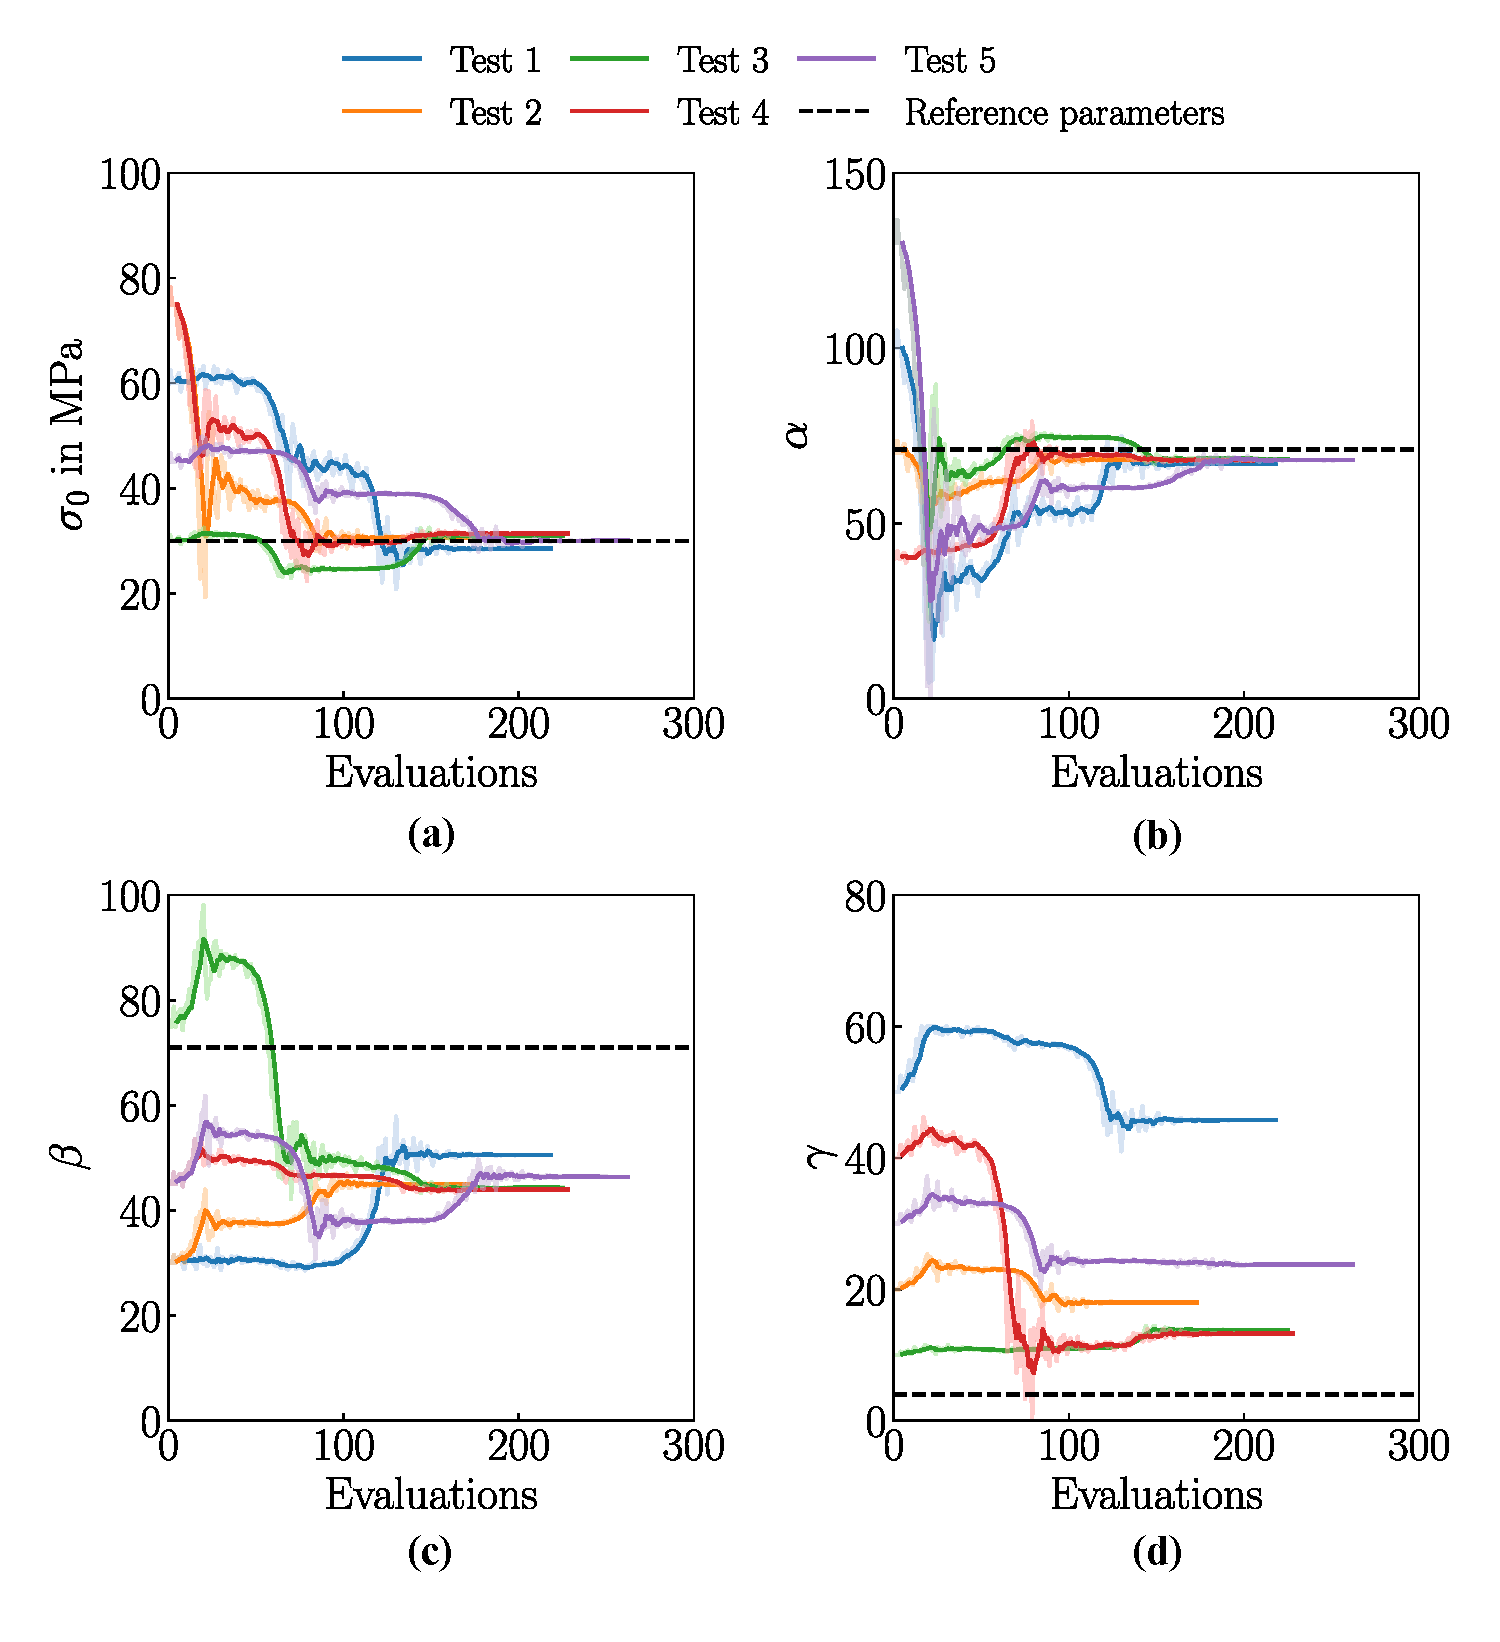
\includegraphics[width=0.66\textwidth]{Vald_4To3_fixEP1_material_params.pdf}
        \caption{Evolution of material 4:3}
        \label{fig:material_params_4to3}
    \end{subfigure}
    \begin{subfigure}[t]{1.0\textwidth}
        \centering
        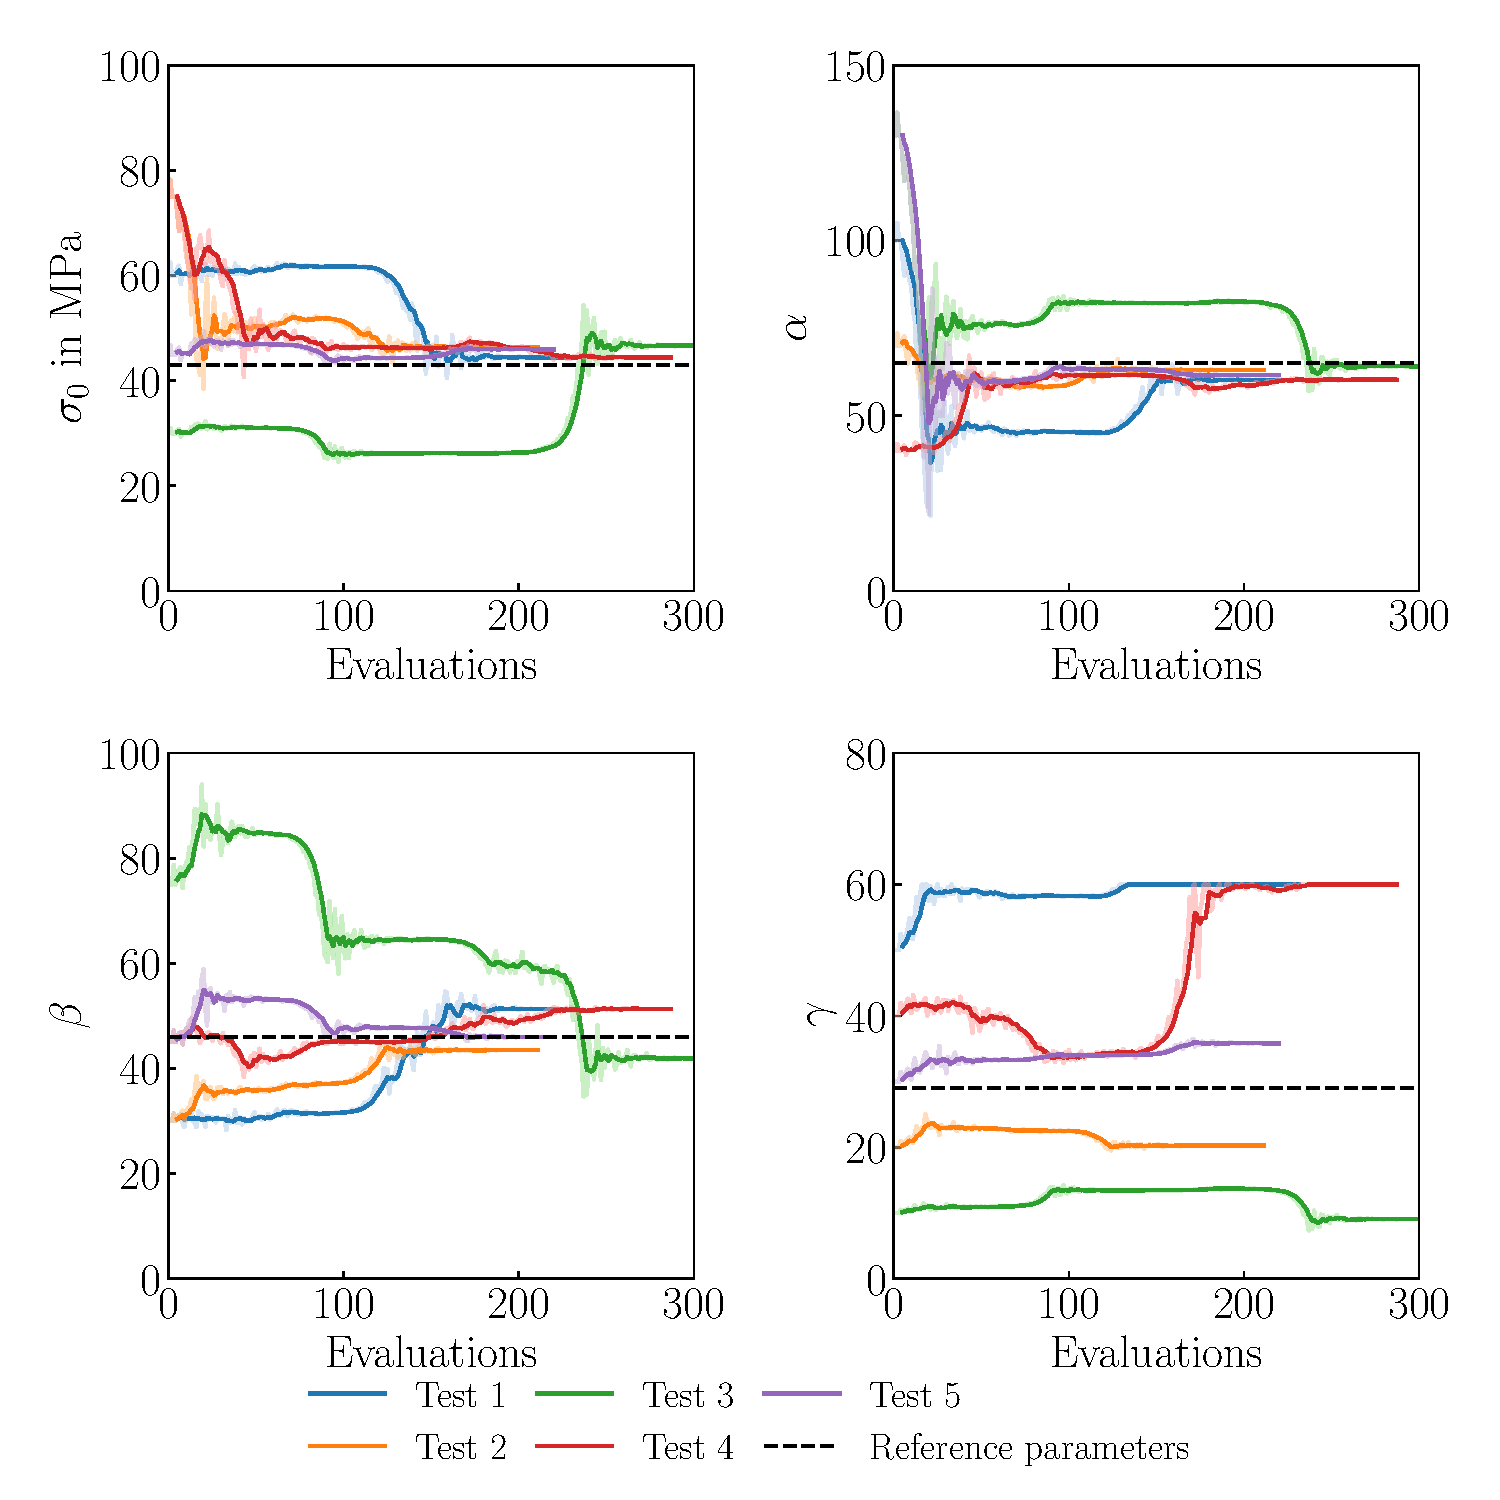
\includegraphics[width=0.66\textwidth]{Vald_8To3_fixEP1_material_params.pdf}
        \caption{Evolution of 8:3}
        \label{fig:material_params_8to3}
    \end{subfigure}
    \caption{Evolution of material parameters for (a) mixing ratio 4:3 and (b) mixing ratio 8:3.}
    \label{fig:validation_material_params}
    \end{figure}

    \begin{figure}[H]
    \centering
    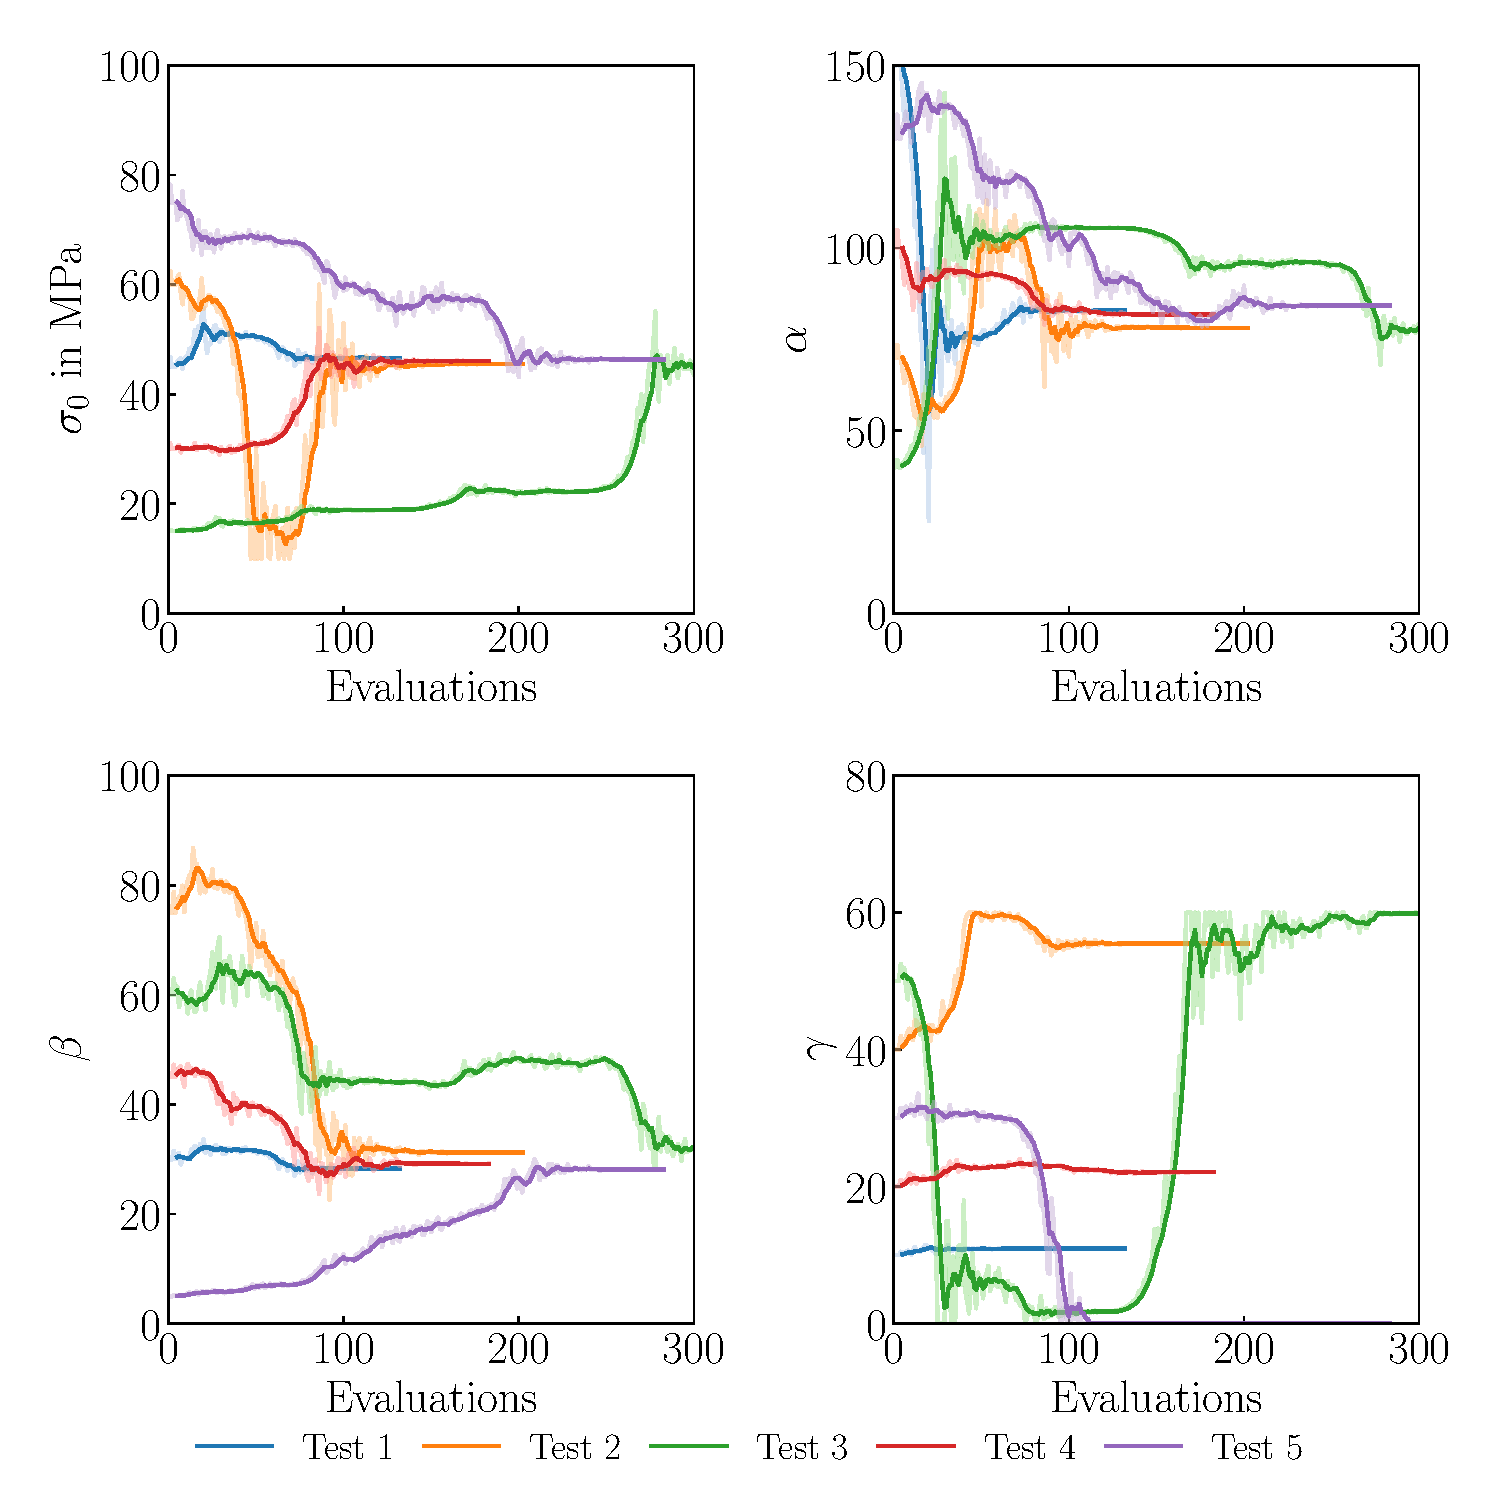
\includegraphics[width=0.7\textwidth]{Tensile_6to3_015_fixENu_material_params.pdf}
    \caption{progress of material parameters for tensile tests}
    \label{fig:tensileMatParams}
    \end{figure}

    \begin{figure}[H]
    \centering
    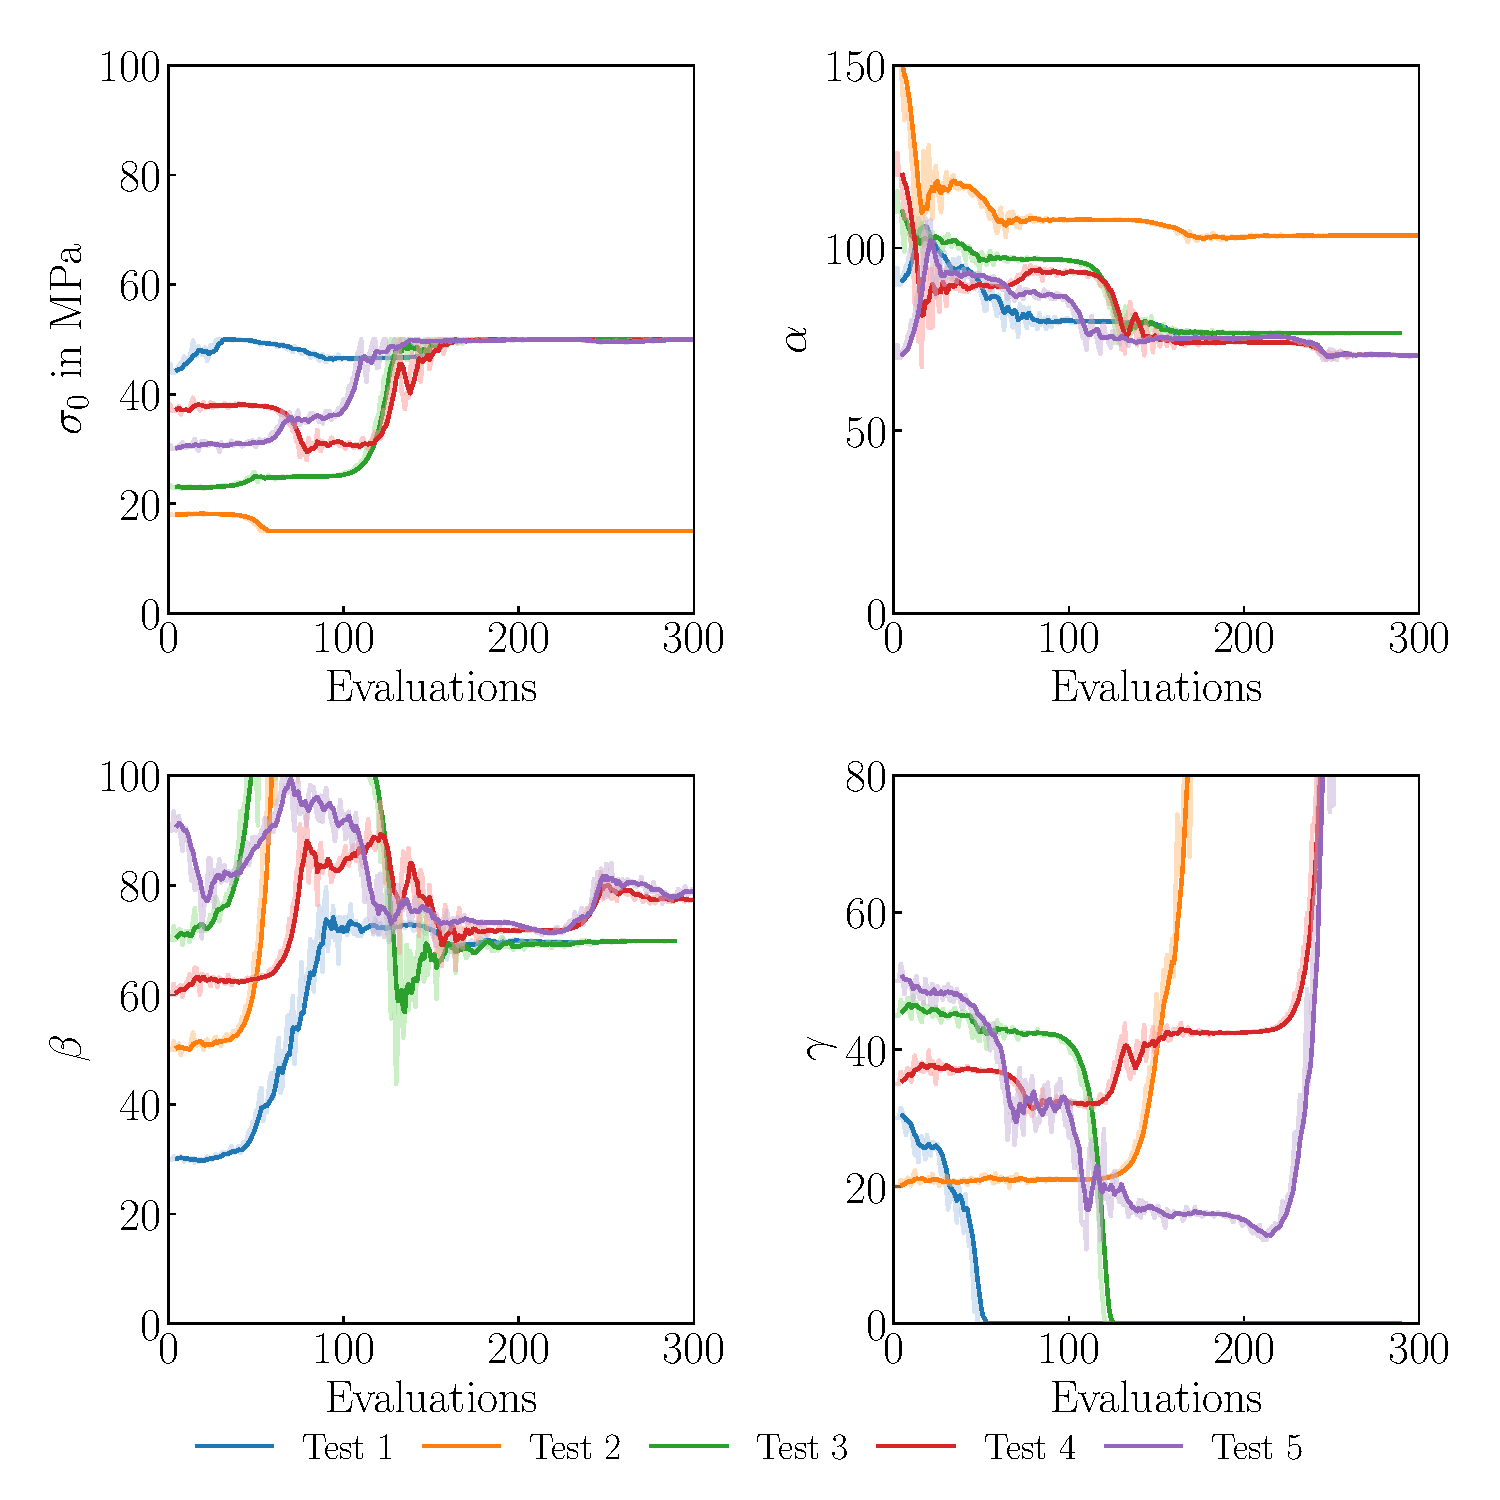
\includegraphics[width=0.7\textwidth]{Shear_6to3_015_fixENu_500_material_params.pdf}
    \caption{progress of material parameters for shear tests}
    \label{fig:shearMatParams}
    \end{figure}


    STRAIN STRAIN PLOTS FÜR VALIDIERUNGSVERSUCHE
    \chapter{Appendix}
\end{appendices}